\documentclass[tikz, border = 5pt]{standalone}
\usepackage{tikz}

\usetikzlibrary{arrows.meta}
\usetikzlibrary{shapes.geometric}

\begin{document}

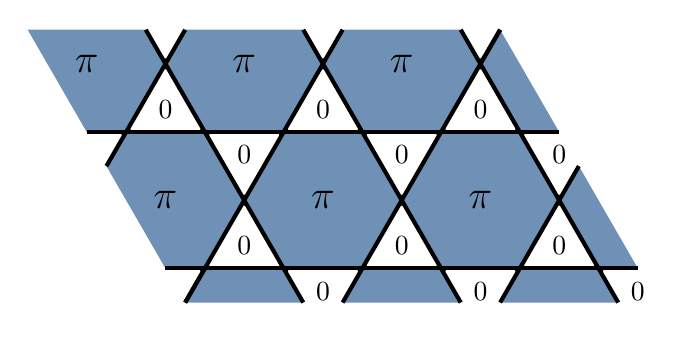
\begin{tikzpicture}[scale = 1.0]

	% model parameters:
	\def \a{1}
	\def \tone{3}
	\def \ttwo{2}
	\def \fs{\Large}

	% artistic parameters:
	\def \lw{1.5pt}

	% colors
	%\definecolor{mypurple}{HTML}{800080}
	\definecolor{mypurple}{HTML}{6F91B5}
	\def \hexcolor{mypurple}

	% get phyical coordinates	
	\newcommand{\getcords}[3]{
	
		\ifnum #3 = 1
			\pgfmathsetmacro{\X}{\a*(2*#1-#2)}
			\pgfmathsetmacro{\Y}{\a*#2*sqrt(3)}
		\else
			\ifnum #3 = 2
				\pgfmathsetmacro{\X}{\a*(2*#1-#2+1)}
				\pgfmathsetmacro{\Y}{\a*#2*sqrt(3)}
			\else
				\pgfmathsetmacro{\X}{\a*(2*#1-#2+0.5)}
				\pgfmathsetmacro{\Y}{\a*sqrt(3)*(#2+1/2)}
			\fi
		\fi
	}
	
	% create lattice points
	\foreach \i in {1,...,\tone}{
		\foreach \j in {1,...,\ttwo}{
			\foreach \l in {1,2,3}{
				\getcords{\i}{\j}{\l}
				\coordinate (P-\i-\j-\l) at (\X, \Y);
				\fill (P-\i-\j-\l) circle (2pt);
			}
		}
	}


	% color hexagons pink 

	\foreach \i in {1,...,\the\numexpr\tone-1\relax}{
		\foreach \j in {1,...,\the\numexpr\ttwo-1\relax}{

			\pgfmathtruncatemacro{\toright}{\i+1}
			\pgfmathtruncatemacro{\up}{\j+1}
			
			\fill[\hexcolor] (P-\i-\j-2) -- (P-\i-\j-3) -- (P-\toright-\up-1) -- (P-\toright-\up-2) -- (P-\toright-\j-3) -- (P-\toright-\j-1) -- cycle;

		}
	}

	% write pi in hexagons


	\foreach \i in {1,...,\the\numexpr\tone-1\relax}{
		\foreach \j in {1,...,\the\numexpr\ttwo-1\relax}{
			\getcords{\i}{\j}{2}
			\pgfmathsetmacro{\Xcord}{\X + 0.5*\a}
			\pgfmathsetmacro{\Ycord}{\Y + sqrt(3)*\a/2}
			\node at (\Xcord, \Ycord) {\fs $\pi$};
		}
	}

	% write 0 in triangles

	\foreach \i in {1,...,\tone}{
		\foreach \j in {1,...,\ttwo}{
			\getcords{\i}{\j}{2}

			\pgfmathsetmacro{\Xcordup}{\X -0.5*\a}
			\pgfmathsetmacro{\Xcorddown}{\X + 0.5*\a}
			\pgfmathsetmacro{\Ycordup}{\Y + \a*0.5/sqrt(3)}
			\pgfmathsetmacro{\Ycorddown}{\Y - \a*0.5/sqrt(3)}

			\node at (\Xcordup, \Ycordup) {$0$};
			\node at (\Xcorddown, \Ycorddown) {$0$};
		}
	}
	

	% color clipped hexagons pink

	% top edge

	\getcords{1}{\ttwo}{1}
	\pgfmathsetmacro{\Xleftbottom}{\X - 0.5*\a}
	\pgfmathsetmacro{\Xlefttop}{\X -1.25*\a}
	\pgfmathsetmacro{\Xrighttop}{\X + 0.25}
	\pgfmathsetmacro{\Ytop}{\Y + 3*sqrt(3)*\a/4}

	\fill[\hexcolor] (P-1-\ttwo-1) -- (P-1-\ttwo-3) -- (\Xrighttop, \Ytop) -- (\Xlefttop, \Ytop) -- (\Xleftbottom, \Y) -- cycle;
	
	\pgfmathsetmacro{\Xcord}{\X - 0.5*\a}
	\pgfmathsetmacro{\Ycord}{\Y + sqrt(3)*\a/2}
	\node at (\Xcord, \Ycord) {\fs $\pi$};

	\foreach \i in {1,...,\the\numexpr\tone-1\relax}{
		
		\getcords{\i}{\ttwo}{2}
		\pgfmathsetmacro{\Ytop}{\Y + 3*sqrt(3)*\a/4}
		\pgfmathsetmacro{\Xleft}{\X - 0.25*\a}
		\pgfmathsetmacro{\Xright}{\X + 1.25*\a}

		\fill[\hexcolor] (P-\i-\ttwo-2) -- (P-\i-\ttwo-3) -- (\Xleft, \Ytop) -- (\Xright, \Ytop) -- (P-\the\numexpr\i+1\relax-\ttwo-3) -- (P-\the\numexpr\i+1\relax-\ttwo-1) -- cycle;

		\pgfmathsetmacro{\Xcord}{\X + 0.5*\a}
		\pgfmathsetmacro{\Ycord}{\Y + sqrt(3)*\a/2}
		\node at (\Xcord, \Ycord) {\fs $\pi$};

	}

	% bottom edge

	\foreach \i in {1,...,\tone}{
		
		\getcords{\i}{1}{1}
		\pgfmathsetmacro{\Xleft}{\X-0.25*\a}
		\pgfmathsetmacro{\Xright}{\X+1.25*\a}
		\pgfmathsetmacro{\Ybottom}{\Y-sqrt(3)*\a/4}

		\fill[\hexcolor] (P-\i-1-1) -- (P-\i-1-2) -- (\Xright, \Ybottom) -- (\Xleft, \Ybottom) -- cycle;
	}

	% right edge

	\foreach \j in {1,...,\ttwo}{

		\getcords{\tone}{\j}{2}
		\pgfmathsetmacro{\Ytop}{\Y + 3*sqrt(3)*\a/4}
		\pgfmathsetmacro{\Xleft}{\X - 0.25*\a}
		\pgfmathsetmacro{\Xright}{\X + 0.5*\a}

		\fill[\hexcolor] (P-\tone-\j-2) -- (P-\tone-\j-3) -- (\Xleft, \Ytop) -- (\Xright, \Y) -- cycle;
	}

	% left edge

	\foreach \j in {1,...,\the\numexpr\ttwo-1\relax}{
		\getcords{1}{\j}{1}
		\pgfmathsetmacro{\Xright}{\X - \a*0.5}
		\pgfmathsetmacro{\Xleft}{\X - \a*1.25}
		\pgfmathsetmacro{\Ytop}{\Y + 3*sqrt(3)*\a/4}

		\fill[\hexcolor] (P-1-\j-1) -- (P-1-\j-3) -- (P-1-\the\numexpr\j+1\relax-2) -- (P-1-\the\numexpr\j+1\relax-1) -- (\Xleft, \Ytop) -- (\Xright, \Y) -- cycle;

		\pgfmathsetmacro{\Xcord}{\X - 0.5*\a}
		\pgfmathsetmacro{\Ycord}{\Y + sqrt(3)*\a/2}
		\node at (\Xcord, \Ycord) {\fs $\pi$};
	}



	% draw nearest nighbour links

	\foreach \i in {1,...,\tone}{
		\foreach \j in {1,...,\ttwo}{
			
			% internal lines
			\draw[line width = \lw] (P-\i-\j-1) -- (P-\i-\j-2);
			\draw[line width = \lw] (P-\i-\j-1) -- (P-\i-\j-3);
			\draw[line width = \lw] (P-\i-\j-2) -- (P-\i-\j-3);

			\ifnum \i < \tone
				\draw[line width = \lw] (P-\i-\j-2) -- (P-\the\numexpr\i+1\relax-\j-1);

				\ifnum \j < \ttwo
					\draw[line width = \lw] (P-\i-\j-3) -- (P-\the\numexpr\i+1\relax-\the\numexpr\j+1\relax-1);
				\fi
			\fi

			\ifnum \j < \ttwo
				\draw[line width = \lw] (P-\i-\j-3) -- (P-\i-\the\numexpr\j+1\relax-2);
			\fi
		}
	}

	% draw half length NN lines at the edge

	% top edge

	\foreach \i in {1,...,\tone}{
		\draw[line width = \lw] (P-\i-\ttwo-3) -- ++ ({0.25*\a}, {sqrt(3)*\a/4});
		\draw[line width = \lw] (P-\i-\ttwo-3) -- ++ ({-0.25*\a}, {sqrt(3)*\a/4});	
	}

	%bottom edge

	\foreach \i in {1,...,\tone}{
		\draw[line width = \lw] (P-\i-1-1) -- ++ ({-0.25*\a}, {-sqrt(3)*\a/4});
		\draw[line width = \lw] (P-\i-1-2) -- ++ ({0.25*\a}, {-sqrt(3)*\a/4});	
	}

	% left edge

	\foreach \j in {1,...,\ttwo}{
		\draw[line width = \lw] (P-1-\j-1) -- ++ ({-0.5*\a},0);
		\draw[line width = \lw] (P-1-\j-1) -- ++ ({-0.25*\a},{-sqrt(3)*\a/4});
	}

	% right edge 

	\foreach \j in {1,...,\ttwo}{
		\draw[line width = \lw] (P-\tone-\j-2) -- ++ ({0.5*\a}, 0);
		\draw[line width = \lw] (P-\tone-\j-3) -- ++ ({0.25*\a}, {sqrt(3)*\a/4});
	}

\end{tikzpicture}

\end{document}
